% Options for packages loaded elsewhere
\PassOptionsToPackage{unicode}{hyperref}
\PassOptionsToPackage{hyphens}{url}
%
\documentclass[
]{book}
\usepackage{amsmath,amssymb}
\usepackage{lmodern}
\usepackage{iftex}
\ifPDFTeX
  \usepackage[T1]{fontenc}
  \usepackage[utf8]{inputenc}
  \usepackage{textcomp} % provide euro and other symbols
\else % if luatex or xetex
  \usepackage{unicode-math}
  \defaultfontfeatures{Scale=MatchLowercase}
  \defaultfontfeatures[\rmfamily]{Ligatures=TeX,Scale=1}
\fi
% Use upquote if available, for straight quotes in verbatim environments
\IfFileExists{upquote.sty}{\usepackage{upquote}}{}
\IfFileExists{microtype.sty}{% use microtype if available
  \usepackage[]{microtype}
  \UseMicrotypeSet[protrusion]{basicmath} % disable protrusion for tt fonts
}{}
\makeatletter
\@ifundefined{KOMAClassName}{% if non-KOMA class
  \IfFileExists{parskip.sty}{%
    \usepackage{parskip}
  }{% else
    \setlength{\parindent}{0pt}
    \setlength{\parskip}{6pt plus 2pt minus 1pt}}
}{% if KOMA class
  \KOMAoptions{parskip=half}}
\makeatother
\usepackage{xcolor}
\usepackage{longtable,booktabs,array}
\usepackage{calc} % for calculating minipage widths
% Correct order of tables after \paragraph or \subparagraph
\usepackage{etoolbox}
\makeatletter
\patchcmd\longtable{\par}{\if@noskipsec\mbox{}\fi\par}{}{}
\makeatother
% Allow footnotes in longtable head/foot
\IfFileExists{footnotehyper.sty}{\usepackage{footnotehyper}}{\usepackage{footnote}}
\makesavenoteenv{longtable}
\usepackage{graphicx}
\makeatletter
\def\maxwidth{\ifdim\Gin@nat@width>\linewidth\linewidth\else\Gin@nat@width\fi}
\def\maxheight{\ifdim\Gin@nat@height>\textheight\textheight\else\Gin@nat@height\fi}
\makeatother
% Scale images if necessary, so that they will not overflow the page
% margins by default, and it is still possible to overwrite the defaults
% using explicit options in \includegraphics[width, height, ...]{}
\setkeys{Gin}{width=\maxwidth,height=\maxheight,keepaspectratio}
% Set default figure placement to htbp
\makeatletter
\def\fps@figure{htbp}
\makeatother
\setlength{\emergencystretch}{3em} % prevent overfull lines
\providecommand{\tightlist}{%
  \setlength{\itemsep}{0pt}\setlength{\parskip}{0pt}}
\setcounter{secnumdepth}{5}
\usepackage{textcomp}
\usepackage{tgbonum}
\usepackage{booktabs}
\usepackage{unixode}
\usepackage{tikz-cd}
\usepackage[catalan]{babel}
\usepackage{amsmath,amsthm,amssymb,amsfonts}
\usepackage[all]{xy}
\definecolor{VerbatimBorderColor}{rgb}{0.7,0.7,0.7}
% from sphinxmanual.cls: put authors on separate lines
\DeclareRobustCommand{\and}{%
\end{tabular}\kern-\tabcolsep\\\begin{tabular}[t]{c}%
}

\usepackage{mathsymbols}
\setlength{\headheight}{15pt}

\makeatletter
\def\thm@space@setup{%
  \thm@preskip=8pt plus 2pt minus 4pt
  \thm@postskip=\thm@preskip
}
\makeatother
\usepackage{textcomp}
\usepackage[unicode=true, breaklinks=true]{hyperref}
\usepackage{lmodern}
\ifLuaTeX
  \usepackage{selnolig}  % disable illegal ligatures
\fi
\usepackage[]{natbib}
\bibliographystyle{apalike}
\nocite{dummitfoote, artinalgebra}
\IfFileExists{bookmark.sty}{\usepackage{bookmark}}{\usepackage{hyperref}}
\IfFileExists{xurl.sty}{\usepackage{xurl}}{} % add URL line breaks if available
\urlstyle{same} % disable monospaced font for URLs
\hypersetup{
  pdftitle={Teoria de Galois},
  pdfauthor={Marc Masdeu},
  hidelinks,
  pdfcreator={LaTeX via pandoc}}

\title{Teoria de Galois}
\author{Marc Masdeu}
\date{2023-02-01}

\usepackage{amsthm}
\newtheorem{theorem}{Teorema}[chapter]
\newtheorem{lemma}{Lema}[chapter]
\newtheorem{corollary}{Corol·lary}[chapter]
\newtheorem{proposition}{Proposició}[chapter]
\newtheorem{conjecture}{Conjectura}[chapter]
\theoremstyle{definition}
\newtheorem{definition}{Definició}[chapter]
\theoremstyle{definition}
\newtheorem{example}{Exemple}[chapter]
\theoremstyle{definition}
\newtheorem{exercise}{Exercici}[chapter]
\theoremstyle{definition}
\newtheorem{hypothesis}{Hipòtesi}[chapter]
\theoremstyle{remark}
\newtheorem*{remark}{Remarca}
\newtheorem*{solution}{Solució}
\begin{document}
\maketitle

{
\setcounter{tocdepth}{1}
\tableofcontents
}
\hypertarget{introducciuxf3}{%
\chapter*{Introducció}\label{introducciuxf3}}
\addcontentsline{toc}{chapter}{Introducció}

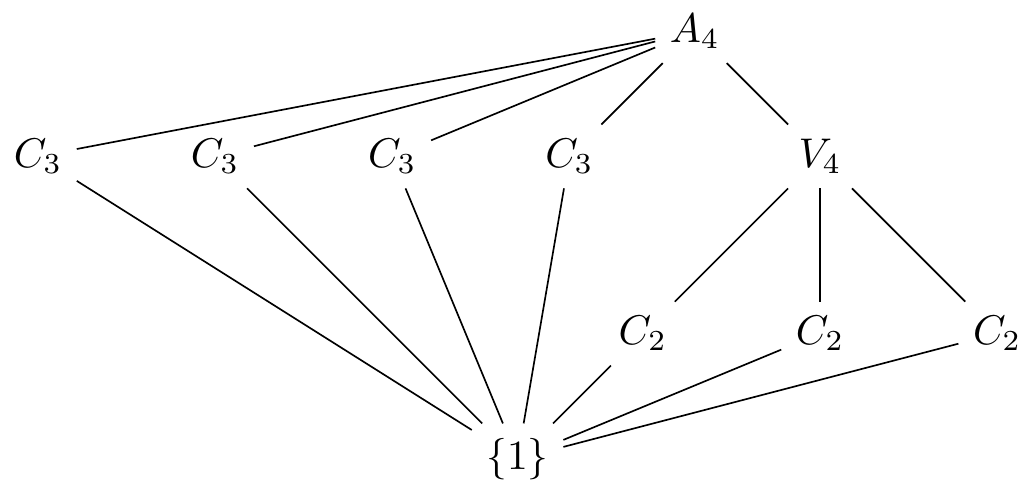
\includegraphics[width=0.7\linewidth]{teoriadegalois_files/figure-latex/unnamed-chunk-1-1}

Aquests són uns apunts de \emph{Teoria de Galois}, pensats pel curs de 3r del Grau de Matemàtiques de la UAB.

L'assignatura de \emph{Teoria de Galois} es cursa al primer semestre del tercer curs del Grau de Matemàtiques de la UAB. Consta de 6 crèdits, repartits en:

\begin{itemize}
\tightlist
\item
  Dues hores setmanals de teoria (15 setmanes), que actualment es fan seguides.
\item
  Una hora setmanal de problemes (15 setmanes).
\item
  Tres seminaris pràctics, de 2h cadascun.
\end{itemize}

El curs es pot dividir de manera natural en 15 sessions de dues hores. El temps efectiu de cadascuna d'aquestes sessions és de 100 minuts, i es pot pensar com una sèrie de 15 capítols. Seguidament detallem cadascun d'aquests capítols i la seva sinopsi.

\hypertarget{pilot}{%
\chapter{Vells coneguts}\label{pilot}}

Començarem recordant les definicions i resultats bàsics que ja s'han vist a altres
assignatures, com Fonaments o Estructures algebraiques. Donarem les definicions de cos,
característica, cos primer, i veurem que aquest és o bé \(\FF_p\) per algun primer \(p\), o bé \(\QQ\).
A continuació introduïrem les extensions de cossos i el grau. Construirem el cos \(F[x]/(p(x))\) associat
a un polinomi irreductible \(p(x)\in F[x]\), i veurem alguns exemples.

\hypertarget{convencions}{%
\section{Convencions}\label{convencions}}

En aquest curs, tots els anells seran commutatius, i assumirem sempre que tenen unitat. A més, demanarem
que un morfisme d'anells enviï l'\(1\) a l'\(1\).

\hypertarget{caracteruxedstica-dun-cos}{%
\section{Característica d'un cos}\label{caracteruxedstica-dun-cos}}

\begin{lemma}
Siguia \(A\) un anell qualsevol. Aleshores hi ha un únic morfisme \(\ZZ \to A\).
\end{lemma}

\begin{proof}
Considerem el morfisme \(\iota\colon \ZZ\to A\) definit com:
\[
\iota(n)=\begin{cases}
1_A+1_A+\cdots+1_A & n \geq 0,\\
-(1_A+1_A+\cdots+1_A) & n < 0,
\end{cases}
\]
on les sumes tenen \(n\) termes. És fàcil comprovar que és un morfisme. La unicitat es demostra per inducció en \(\abs{n}\).
\end{proof}

A partir d'ara, qualsevol enter el podem pensar com a element d'un anell donat, i això no ens portarà cap confusió. Com ja sabem, el nucli d'un morfisme d'anells és un ideal. Per tant, el nucli del morfisme \(\iota_A\colon \ZZ\to A\) és un ideal de \(\ZZ\) de
la forma \((n)\), amb \(n\geq 0\).

\begin{definition}[Característica]
La \emph{característica} d'un anell \(A\) és l'enter no negatiu \(n\) tal que \(\iota_A = (n)\), i es denota per \(\car(A)\).
\end{definition}

Fixem-nos que si \(\car(A)=n\), aleshores \(na = 0\) per a tot \(a\in A\).

\begin{proposition}
\protect\hypertarget{prp:car-primer}{}\label{prp:car-primer}Sigui \(F\) un cos. Aleshores la seva característica és \(0\) o bé un primer \(p\).
\end{proposition}

\begin{proof}
Suposem que \(\car(F)=n>0\), i \(n=ab\). Aleshores \((a1_A)(b1_A)=(ab)1_A=0\). Com que \(F\) és un cos,
això vol dir que \(a1_A=0\) o \(b1_A=0\). Si per exemple \(a1_A=0\), això significa que \(n \mid a\). Com que \(n=ab\),
necessàriament \(a=n\) i \(b=1\). Per tant, els únics divisors de \(n\) són trivials, i \(n\) és primer.
\end{proof}

\begin{definition}[cos primer]
\protect\hypertarget{def:cos-primer}{}\label{def:cos-primer}El \emph{cos primer} d'un cos \(F\) és el cos generat per \(1_F\). És o bé \(\QQ\) (si \(F\) té característica \(0\)) o bé el cos \(\FF_p\)
(si \(F\) té característica \(p\)).
\end{definition}

\hypertarget{extensions}{%
\section{Extensions}\label{extensions}}

Quan \(K\) és un cos que conté un altre cos \(F\), direm que \(K\) és una \emph{extensió} de \(F\), i escriurem \(K/F\) (no és cap mena de quocient!). Direm també que
\(F\) és el \emph{cos base} de l'extensió \(K/F\). També farem servir
el diagrama
\[
\begin{xy}
\xymatrix{
  K\ar@{-}[d]\\
  F.
}
\end{xy}
\]

Com que un cos no té ideals propis, un morfisme de cossos \(\iota\colon F\to K\) és sempre injectiu i, per tant, la
imatge de \(\iota\) és un subcos de \(K\) isomorf a \(F\). A partir d'ara, a vegades identificarem \(F\) amb \(\iota(F)\), i direm
que \(K\) és una extensió de \(F\).

Seguidament fem la següent observació clau: quan tenim una extensió \(K/F\) aleshores \(K\) esdevé automàticament un \(F\)-espai vectorial. Això
ens permet definir:

\begin{definition}[grau d'una extensió]
\protect\hypertarget{def:grau-ext}{}\label{def:grau-ext}El \emph{grau} de l'extensió \(K/F\) és la dimensió de \(K\) com a \(F\)-espai vectorial, que escrivim com \([K\colon F]\). Direm que \(K/F\) és finita si té grau finit,
i infinita si no.
\end{definition}

\begin{theorem}[adjunció d'arrels]
\protect\hypertarget{thm:ext-arrel}{}\label{thm:ext-arrel}Sigui \(p(x)\in F[x]\) un polinomi irreductible. Aleshores existeix una extensió \(K/F\) tal que \(K\) té una arrel de \(p(x)\).
\end{theorem}

\begin{proof}
TODO
\end{proof}

El següent teorema ens diu que l'extensió donada pel teorema anterior té grau igual al grau del polinomi (per això s'ha triat
el nom!). De fet, ens dona una base de \(K\) com a \(F\)-espai vectorial.

\begin{theorem}
\protect\hypertarget{thm:ext-arrel-base}{}\label{thm:ext-arrel-base}Sigui \(p(x)\in F[x]\) un polinomi irreductible de grau \(n\), i sigui \(K=F[x]/(p(x))\). Sigui \(\alpha\) la classe de \(x\) a \(K\).
Aleshores els elements \((1,\alpha,\ldots,\alpha^{n-1})\) formen una \(F\)-base de \(K\).
\end{theorem}

\begin{proof}
TODO
\end{proof}

L'aritmètica a \(F[x]/(p(x))\) és molt explícita: els seus elements es poden expressar com a polinomis en \(\alpha\) de grau
menor que \(n=\deg(p(x))\). Donats dos polinomis \(a(\alpha)\) per \(b(\alpha)\), podem considerar
el residu \(r(x)\) de dividir \(a(x)b(x)\) per \(p(x)\). Aleshores el producte \(a(\alpha)b(\alpha)\) ve donat per l'element \(r(\alpha)\).
Per divir ens cal utilitzar la identitat de Bézout (exercici).

\begin{example}
Mostrem \(\CC\) com el resultat d'adjuntar una arrel de \(x^2+1\) a \(\RR\).
\end{example}

\begin{example}
Podem construir de manera semblant \(\QQ(i)\), o \(\QQ(\sqrt{2})\), i també \(\QQ(\sqrt[3]{2})\). Veurem com es
poden fer les operacions habituals en algun d'aquests cossos.
\end{example}

\begin{example}
Si considerem \(\FF_p\) el cos finit de \(p\) elements i un polinomi \(f(x)\in \FF_p[x]\) irreductible de grau \(n\)
(suposant que existeixi!), aleshores obtenim un cos \(K/\FF_p\) de grau \(n\). Té, per tant, \(p^n\) elements.
\end{example}

\begin{example}
També podem fer extensions de cossos més ``exòtics''. Per exemple, podem prendre \(k(t)\) com el cos de funcions
racionals sobre un cos fixat \(k\), i ``afegir'' una arrel quadrada de \(t\) (mitjançant el polinomi \(x^2-t\)).
\end{example}

Sigui \(K/F\) una extensió, i considerem un conjunt \(S\subseteq K\). Aleshores podem considerar el ``mínim'' subcos \(L\subseteq K\)
que conté \(F\) i tots els elements de \(S\). S'anomena el \emph{cos generat per \(S\) sobre \(F\)}, i escriurem \(F(S)\). Si \(S\) és un
conjunt finit format per \(\alpha_1,\ldots,\alpha_n\) aleshores escriurem \(F(\alpha_1,\ldots,\alpha_n)\). Un cas particular
és quan \(S\) conté un sol element: en aquest cas \(F(\alpha)\) s'anomena una extensió \emph{simple}, i l'element \(\alpha\) s'anomena
un \emph{element primitiu} de l'extensió (que no és únic, en general!).

\begin{theorem}[extensió simple]
\protect\hypertarget{thm:ext-simple}{}\label{thm:ext-simple}Sigui \(p(x)\in F[x]\) un polinomi irreductible, i suposem que \(K/F\) és una extensió que conté una arrel \(\alpha\) de \(p(x)\).
Aleshores hi ha un isomorfisme \[F[x]/(p(x))\cong F(\alpha).\]
Aquest isomorfisme és únic si demanem que \([x]\mapsto \alpha\).
\end{theorem}

\begin{proof}
TODO
\end{proof}

\begin{example}
Expliquem l'exemple de \(\QQ(\sqrt{2})\) i la diferència amb \(\QQ(\sqrt[3]{2})\). Aquest darrer cos és un subcòs de \(\RR\), però hi ha
un altre subcòs de \(\CC\) que és isomorf a aquest.
\end{example}

\begin{remark}[]
En els exemples, hem construit cossos que contenen una de les tres possibles arrels de \(x^3-2\). Aquests són isomorfs, tal
i com hem vist. El fet que un sigui subcos de \(\RR\) i l'altre de \(\CC\) té a veure amb anàlisi, no amb àlgebra. Algebraicament,
no es poden distingir.
\end{remark}

Acabem amb un teorema que ens servirà més endavant:

\begin{theorem}[extensió d'isomorfismes]
Sigui \(\varphi\colon F\to \tilde F\) un isomorfisme de cossos. Sigui \(p(x)\in F[x]\) un polinomi irreductible,
i sigui \(\tilde p(x)\) el polinomi resultant d'aplicar \(\varphi\) als coeficients de \(p(x)\). Sigui \(\alpha\) una
arrel de \(p(x)\) en alguna extensió de \(K\), i sigui \(\beta\) una arrel de \(\tilde p(x)\) en una extensió de \(\tilde F\).
Aleshores l'aplicació \(\alpha\mapsto \beta\) indueix un isomorfisme de cossos
\[
\Phi\colon F(\alpha) \cong \tilde F(\beta)
\]
tal que \(\Phi_{| F} = \varphi\):
\[
\begin{xy}
\xymatrix{
  F(\alpha)\ar_{\cong}^{\Phi}[r]\ar@{-}[d] & \tilde F(\beta)\ar@{-}[d]\\
  F \ar_{\cong}^{\varphi}[r] & \tilde F.
}
\end{xy}
\]
\end{theorem}

\hypertarget{les-torres}{%
\chapter{Les Torres}\label{les-torres}}

Parlarem d'extensions simples, del teorema d'aixecament a anells de polinomis i el teorema de l'extensió.
També definirem elements algebraics i transcendents i el polinomi mínim d'un element algebraic, amb exemples.
Enunciarem i demostrarem la fórmula de les torres, i com es comporta el grau en composicions de cossos.

\hypertarget{extensions-algebraiquestranscendents}{%
\section{Extensions algebraiques/transcendents}\label{extensions-algebraiquestranscendents}}

Considerem una extensió \(K/F\).

\begin{definition}[element algebraic]
Diem que un element \(\alpha\in K\) és \emph{algebraic sobre \(F\)} si \(\alpha\) és l'arrel d'un polinomi \(f(x)\in F[x]\).

Diem que \(\alpha\) és \emph{transcendent sobre \(F\)} si no és algebraic.

L'extensió \(K/F\) és \emph{algebraica} si tots els elements \(\alpha\in K\) són algebraics sobre \(F\).
\end{definition}

Fixem-nos que si \(\alpha\) és algebraic sobre \(F\) aleshores sabem que hi ha \emph{algun} polinomi \(f(x)\in F[x]\) que té \(\alpha\)
com a arrel. Però n'hi ha molts més, per exemple qualsevol múltiple de \(f(x)\). El següent resultat ens permet assignar un
polinomi \emph{canònic} a cada element algebraic.

\begin{proposition}
Si \(\alpha\) és algebraic sobre \(F\), aleshores hi ha un únic polinomi \textbf{mònic} i \textbf{irreductible} \(\Irr_{\alpha,F}(x)\) que
té \(\alpha\) com a arrel. A més, \(f(x)\in F[x]\) té \(\alpha\) com a arrel si i només si és un múltiple de \(\Irr_{\alpha, F}(x)\).
\end{proposition}

\begin{proof}
TODO
\end{proof}

Fixem-nos que, si \(K/L/F\) és una torre d'extensions i \(\alpha\in K\) és algebraic sobre \(F\), aleshores també ho és sobre \(L\),
i a més \(\Irr_{\alpha,L}(x)\) divideix \(\Irr_{\alpha,F}(x)\) a \(L[x]\).

\begin{definition}[polinomi mínim]
El polinomi \(\Irr_{\alpha,F}(x)\) s'anomena el \emph{polinomi mínim d'\(\alpha\) sobre \(F\)}, i el seu grau s'anomena el \emph{grau d'\(\alpha\)}
sobre \(F\).
\end{definition}

Posant junt tot el què hem vist fins ara, si prenem \(\alpha\in K\) aleshores podem considerar a subextensió \(F(\alpha)/F\).
En aquest cas, \(F(\alpha)\cong F[x]/(\Irr_{\alpha,F}(x))\) i per tant \([F(\alpha)\colon F] = \deg \alpha\).

\begin{example}
Revisitem els exemples anteriors, calculant els seus polinomis mínims.
\end{example}

\begin{proposition}
Si \([K\colon F]=n\) i \(\alpha\in K\), aleshores \(\deg\alpha\leq n\). En particular, \(K/F\) és algebraica.
\end{proposition}

\begin{proof}
TODO
\end{proof}

No és cert que tota extensió algebraica sigui finita (en veurem exemples més endavant).

El següent resultat ens caracteritza com són les extensions quadràtiques d'un cos \(F\) de característica \(\neq 2\).

\begin{proposition}[]
Sigui \(F\) un cos de característica \(\neq 2\), i sigui \(K/F\) una extensió de grau \(2\). Aleshores existeix \(\delta\in K\setminus F\)
tal que \(\delta^2=D\in F\) i \(K=F(\delta)\). Escriurem que \(K=F(\sqrt{D})\).
\end{proposition}

\begin{proof}
TODO
\end{proof}

\hypertarget{torres-de-cossos}{%
\section{Torres de cossos}\label{torres-de-cossos}}

En aquesta secció considerem torres \(L/K/F\). Ens interessa relacionar les dues extensions \(L/K\) i \(K/F\) amb l'extensió
total \(L/F\).

\begin{theorem}[fórmula de les torres]
\protect\hypertarget{thm:torres}{}\label{thm:torres}Si \(F\subseteq K\subseteq L\), aleshores
\[
[L\colon F] = [L\colon K][K \colon F].
\]
Si un costat de l'equació és infinit, aleshores l'altre també.
\end{theorem}

\begin{proof}
TODO (fàcil, però poc elegant)
\end{proof}

\begin{corollary}
Si \(L/F\) és una extensió finita i \(K/F\) és una subextensió (és a dir, K\subseteq L\$) aleshores \([K\colon F]\) divideix \([L\colon F]\).
\end{corollary}

Per exemple, el corol·lari anterior ens permet deduïr que \(\sqrt{2}\) no pertany a cap extensió de grau senar.

\begin{exercise}
Demostreu que el polomi \(x^3-\sqrt{2}\) és irreductible sobre \(\QQ(\sqrt{2})\).
\end{exercise}

\hypertarget{regle-i-compuxe0s}{%
\chapter{Regle i Compàs}\label{regle-i-compuxe0s}}

Parlarem de tres problemes de la grècia clàssica sobre construccions amb regle no marcat i compàs: la quadratura del cercle,
la trisecció de l'angle i la duplicació del cub. Caracteritzarem els nombres constructibles, i veurem que aquests problemes
no tenen solució. Veurem també que si el regle és marcat aleshores podem trisecar l'angle i també duplicar el cub.

\hypertarget{descomposiciuxf3}{%
\chapter{Descomposició}\label{descomposiciuxf3}}

El cos de descomposició d'un polinomi juga un paper destacat al llarg del curs.
Aquí el definirem, i en demostrarem l'existència i unicitat (llevat d'isomorfisme).
Aprofitarem per definir extensions normals (aquelles que són cos de descomposició d'un conjunt de polinomis).

Com a aplicació, s'introduiran els polinomis i cossos ciclotòmics, i ho lligarem amb la
demostració de l'existència i unicitat de cossos finits de cardinal potència d'un primer.

També veurem les clausures algebraiques, i una construcció (seguint Artin). Això ens permetrà (assumint el teorema fonamental
de l'àlgebra, que demostrarem més endavant) pensar els elements algebraics sobre \(\QQ\) dins dels complexos.

\hypertarget{polinomis-inseparables}{%
\chapter{Polinomis Inseparables}\label{polinomis-inseparables}}

Definim la noció de separabilitat d'un polinomi, i posem algun exemple. Introduïm el morfisme de Frobenius,
que ens permet definir cossos perfectes. Aprofitem per parlar del grau de separabilitat/inseparabilitat d'una
extensió, i la factorització d'aquesta.

Finalment, donem l'existència i unicitat dels cossos finits.

\hypertarget{polinomis-ciclotuxf2mics}{%
\chapter{Polinomis Ciclotòmics}\label{polinomis-ciclotuxf2mics}}

L'objectiu principal és demostrar que l'extensió ciclotòmica \(\QQ(\zeta_n)\) té grau \(\varphi(n)\) (la phi d'Euler). Per això,
introduïrem els polinomis ciclotòmics, veurem que són irreductibles i mònics i tenen coeficients enters.

\hypertarget{automorfismes}{%
\chapter{Automorfismes}\label{automorfismes}}

Aquesta sessió no parla de teoria de cossos, sinó de grups. Això ens cal ja que el teorema fonamental ens relaciona les dues teories. Introduïrem
la noció de resolubilitat d'un grup, parlarem dels grups simples i veurem que el grup alternat \(A_n\) no és simple per a tot \(n \geq 5\). Això
implica que \(S_n\) no és resoluble per \(n\geq 5\).

Començarem definint els automorfismes d'una extensió. Veurem que formen
un grup, i que cada subgrup té associat el cos dels elements fixos per aquest. Veurem també
que els automorfismes envien cada element \(\alpha\) a una arrel de \(\Irr(\alpha,x)\),
i demostrarem que en una extensió normal el cardinal del grup d'automorfismes està
fitat pel grau de l'extensió. Així, podrem definir una extensió de Galois com aquella
on la fita s'assoleix.

\hypertarget{el-teorema-fonamental}{%
\chapter{El Teorema Fonamental}\label{el-teorema-fonamental}}

Enunciem i demostrem el teorema fonamental de la teoria de Galois. Farem
servir la independència lineal dels caràcters (que tmabé demostrarem). Després veurem
que si \(L / F\) és una extensió finita i \(H\) un subgrup de \(\Aut(L/F)\), aleshores
\([L \colon FH] = |H|\). Aquest fet, fonamental, ens permet també caracteritzar
les extensions de Galois com aquelles que són normals i separables.

Aleshores ja estarem en posició d'enunciar i demostrar el teorema fonamental. Acabarem
amb diversos exemples concrets d'extensions, il·lustrant la correspondència de Galois.

\hypertarget{la-independuxe8ncia-dels-caruxe0cters}{%
\section{La independència (dels caràcters)}\label{la-independuxe8ncia-dels-caruxe0cters}}

En aquesta secció demostrarem un resultat d'àlgebra lineal necessari per la demostració del teorema fonamental de la TG.

\begin{definition}
\protect\hypertarget{def:caracter}{}\label{def:caracter}Un \emph{caràcter} \(\chi\) d'un grup \(G\) amb valors en un cos \(L\) és un morfisme de grups
\[
\chi \colon G \to L^\times.
\]
\end{definition}

Podem pensar un caràcter \(\chi\) com una funció \(G\to L\). Les funcions de \(G\) a \(L\) formen un \(L\)-espai vectorial, de manera òbvia.

\begin{theorem}[Independència lineal dels caràcters]
\protect\hypertarget{thm:caracters-li}{}\label{thm:caracters-li}Siguin \(\chi_1,\ldots,\chi_n\) caràcters de \(G\) diferents. Aleshores són linealment independents, és a dir, no hi ha
cap combinació lineal no trivial \(a_1\chi_1+\cdots+a_n\chi_n\) que doni lloc a la funció idènticament zero.
\end{theorem}

\begin{proof}
Suposem (reordenant, si cal) que podem escriure
\[
a_1\chi_1 + \cdots a_m\chi_m = 0,
\]
amb tots els \(a_i\neq 0\) (observem \(m\leq n\)) i amb \(m\) mínim. Obtindrem una relació de dependència amb menys termes, arribant així a contradicció.

Prenem \(g_0\in G\) tal que \(\chi_1(g_0)\neq \chi_m(g_0)\). Aleshores tenim
\[
a_1\chi_1(g) + \cdots a_m\chi_m(g) = 0,
\]
i
\[
a_1\chi_1(g_0g) + \cdots a_m\chi_m(g_0g) = 0.
\]
Multiplicant la primera equació per \(\chi_m(g_0)\) i restant-li la segona obtenim, per a tot \(g\),
\[
a_1(\chi_m(g_0)-\chi_1(g_0)) \chi_1(g) + \cdots a_{m-1}(\chi_m(g_0)- \chi_{m-1}(g_0)) \chi_{m-1}(g) = 0.
\]
Com que el primer coeficient és diferent de zero, tenim una relació no trivial amb \(m-1\) termes, contradicció.
\end{proof}

Un cas particular que ens interessa aquí prové de consirar un morfisme no trivial de cossos \(\sigma\colon K\to L\),
que indueix un morfisme de grups entre les unitats \(\sigma\colon K^\times \to L^\times\) (aquesta restricció ja conté
tota la informació que ens cal de \(\sigma\), perquè ja sabem que \(\sigma(0)=0\)). Aleshores \(\sigma\) esdevé un caràcter
del grup \(G=K^\times\), i per tant tenim el següent:

\begin{corollary}
Si \(\sigma_1,\ldots,\sigma_n\) són morfismes diferents de \(K\) a \(L\), aleshores són linealment independents com a funcions de \(K\).
\end{corollary}

Un cas encara més particular d'aquest corol·lari ens permet demostrar una relació numèrica bàsica entre automorfismes d'un cos
i els cossos que deixen fixes.

\begin{proposition}
Sigui \(S\) un subconjunt finit d'automorfismes d'un cos \(K\), i sigui \(F=K^G\) el seu cos fix. Aleshores
\[
[K\colon F] \geq |S|.
\]
\end{proposition}

\begin{proof}
TODO
\end{proof}

\begin{theorem}
Sigui \(G\) un subgrup finit d'automorfismes d'un cos \(K\), i sigui \(F=K^G\) el seu cos fix. Aleshores
\[
[K\colon F] = |G|.
\]
\end{theorem}

\begin{proof}
Només ens cal veure que \([K\colon F] \leq |G|\), ja que l'altra desigualtat ja l'hem demostrat independentment
del fet que \(G\) sigui un grup.

TODO (llarga)
\end{proof}

D'aquest resultat se'n desprenen fàcilment conseqüències molt importants que val la pena destacar.

\begin{corollary}
Si \(K/F\) és una extensió finita, aleshores
\[
|\Aut(K/F)| \leq [K\colon F],
\]
amb igualtat si i només si \(F\) és el cos fix d'\(\Aut(K/F)\).
\end{corollary}

Dit d'altra manera, l'extensió \(K/F\) és Galois si i només si \(F=K^{\Aut(K/F)}\).

\begin{proof}
TODO.
\end{proof}

\hypertarget{cossos-finits}{%
\chapter{Cossos Finits}\label{cossos-finits}}

\hypertarget{lelement-primitiu}{%
\chapter{L'element Primitiu}\label{lelement-primitiu}}

\hypertarget{extensions-abelianes-i-ciclotuxf2miques}{%
\chapter{Extensions Abelianes i ciclotòmiques}\label{extensions-abelianes-i-ciclotuxf2miques}}

En aquest apartat estudiem les extensions ciclotòmiques, i veiem que \(\Gal(\QQ(\zeta_n))\)
és canònicament isomorf a \((\ZZ/n\ZZ)^\times\). Com a aplicació, veurem com construir
polígons regulars amb regle i compàs. Veurem que només és possible per polígons regulars
de \(n\) costats quan \(\varphi{n}\) és una potència de \(2\). Això passa si i només si \(n\) és producte
d'una potència de dos i de primers de Fermat diferents.

\hypertarget{arrels-i-radicals}{%
\chapter{Arrels i radicals}\label{arrels-i-radicals}}

Definirem què vol dir que un polinomi sigui resoluble per radicals, i veurem
que és equivalent a què el seu grup de Galois sigui resoluble. D'aquí en podrem
deduir que els polinomis generals de grau \(\geq 5\) no són resolubles per radicals i,
per tant, no existeix una fórmula que expressi les arrels d'un polinomi en termes
dels seus coeficients. També es mostrarà un exemple concret d'un polinomi de grau \(5\) sobre \(\QQ\)
amb grup de Galois \(S_5\).

\begin{proposition}[]
Sigui \(f(x)\in \QQ[x]\) un polinomi irreductible de grau \(p\) amb exactament \(p-2\) arrels reals. Aleshores \(\Gal(f)\cong S_p\).
\end{proposition}

\begin{proof}
TODO
\end{proof}

Podem aplicar el resultat anterior al polinomi \(f(x)=x^5-4x-2\). Com que és \(2\)-Eisenstein, és irreductible. A més, la seva derivada
és \(5x^4-4\), que té zeros a \(x=\pm\frac{\sqrt{2}}{\sqrt[4]{5}}\). Deduïm que \(f(x)\) té exactament tres zeros reals,
que de fet podem aproximar: \(-1.24359639\ldots,-0.50849948\ldots,1.51851215\ldots\). Per tant, \(\Gal(f)\cong S_5\).

\hypertarget{calculem-grups-de-galois}{%
\chapter{Calculem grups de Galois}\label{calculem-grups-de-galois}}

\nocite{*}

  \bibliography{src/bibliografia.bib}

\end{document}
